%En el grafico se puede observar como el crecimiento de todos las heuristicas es polinomial a menida que el grafo aumenta su densidad en aristas. A su vez el algoritmo $Tabu$ $Search$ presenta una mayor diferencia en cuanto a tiempo, esto es razonable porque puede empeorar parcialmente la solucion dependiendo la cantidad de nodos, entonces esa diferencia (constante) lo que hace es "subirme" la funcion la cantidad observada. 

Para realizar la experimentación respecto a la calidad de las heurísticas presentadas, utilizamos un generador de las siguientes familias de grafos:
\begin{itemize}
\item Estrella + CMF
 \begin{figure}[H] %[h] Aqui [b] para button [t] para top
\begin{center}
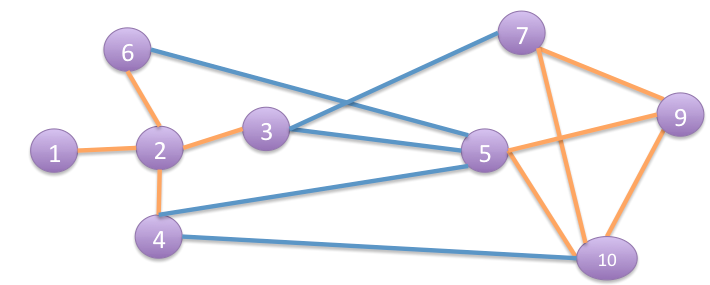
\includegraphics[width=200pt]{../imgs/Estrella+CMF.jpg}
\caption{Grafo de ejemplo de tipo Estrella con una CMF que no esta en la estrella.}
\end{center}
\end{figure}
\item Estrella+Puente+CMF
 \begin{figure}[H] %[h] Aqui [b] para button [t] para top
\begin{center}
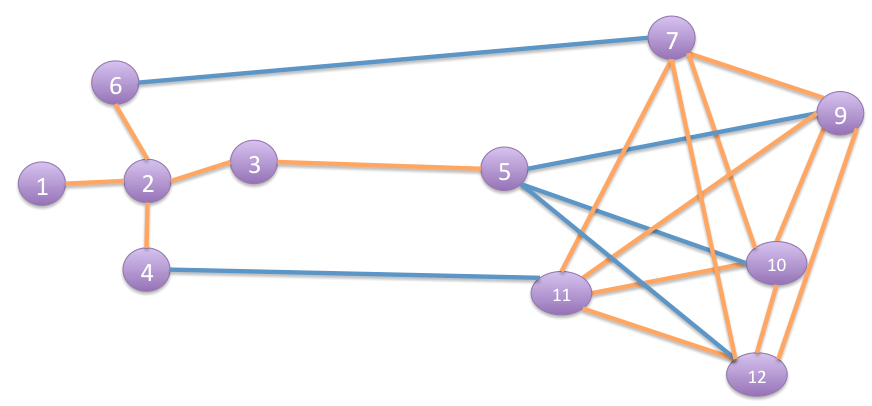
\includegraphics[width=200pt]{../imgs/Estrella+Puente+CMF.jpg}
\caption{Grafo de ejemplo de tipo Estrella con un puente a otra parte del grafo que tiene la CMF}
\end{center}
\end{figure}
\item Estrella+Puente+Doble Estrella
 \begin{figure}[H] %[h] Aqui [b] para button [t] para top
\begin{center}
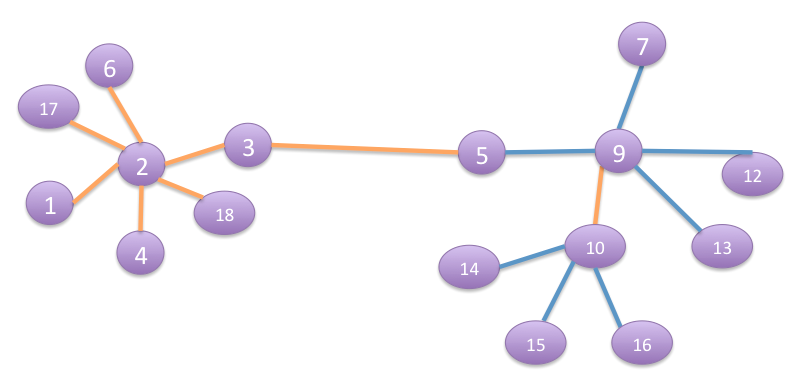
\includegraphics[width=200pt]{../imgs/Estrella+puente+dobleEstrella.jpg}
\caption{Grafo de ejemplo de tipo Estrella con un puente a una estrella doble.}
\end{center}
\end{figure}

\item Banana Tree (Palmera)
 \begin{figure}[H] %[h] Aqui [b] para button [t] para top
\begin{center}
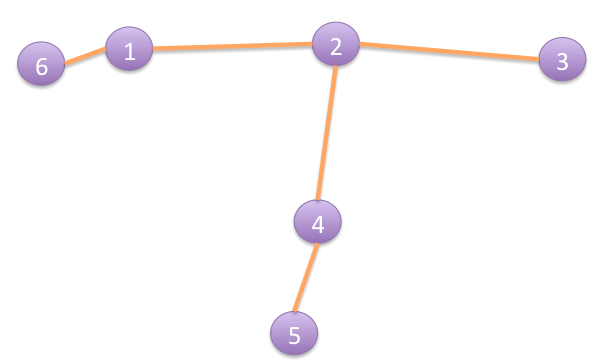
\includegraphics[width=200pt]{../imgs/banana.jpg}
\caption{Grafo de ejemplo de tipo Estrella con un puente a una estrella doble.}
\end{center}
\end{figure}
\item Rueda
 \begin{figure}[H] %[h] Aqui [b] para button [t] para top
\begin{center}
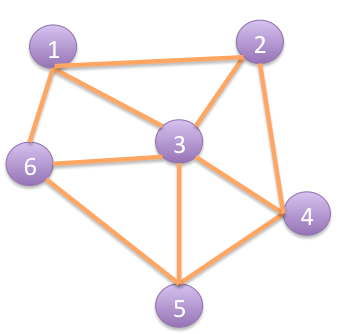
\includegraphics[width=150pt]{../imgs/rueda.jpg}
\caption{Grafo de ejemplo de tipo Estrella con un puente a una estrella doble.}
\end{center}
\end{figure}
\end{itemize}
Luego, procedimos aumentando la cantidad de nodos de los grafos, que a su vez aumenta la cantidad de aristas de éstos dado que los grafos en cuestión se caracterizan por un porcentaje determinado de aristas con respecto a sus nodos. De este modo, realizamos pruebas para cada heurística sobre cada familia de grafos.

Por otro lado, separamos las pruebas de calidad de soluciones en chicas y grandes, esto lo hicimos ya que nos interesa ver la solucion obtenida por el algoritmo exacto para poder compararlo con las heurísticas, y en otro contexto tambien comparar la calidad de las soluciones de las heurísticas para grafos donde el algoritmo exacto no puede resolver a tiempo. 

Las pruebas chicas consisten en grafos de entre 10 y 150 nodos con una densidad de aristas del 50\%. De esta forma, el algoritmo exacto puede encontrar soluciones en un tiempo relativamente rápido y nos permite compararlo con las heurísticas. En el caso de las pruebas grandes, tomamos grafos de entre 200 y 2000 nodos con una densidad de aristas del 50\%. La decisión acerca de la cantidad de aristas se realizó de forma tal a encontrar un balance entre grafos con pocas y muchas aristas, sin afectar demasiado el tiempo de ejecución del algoritmo exacto y de las heurísticas. 


 \begin{figure}[H] %[h] Aqui [b] para button [t] para top
\begin{center}
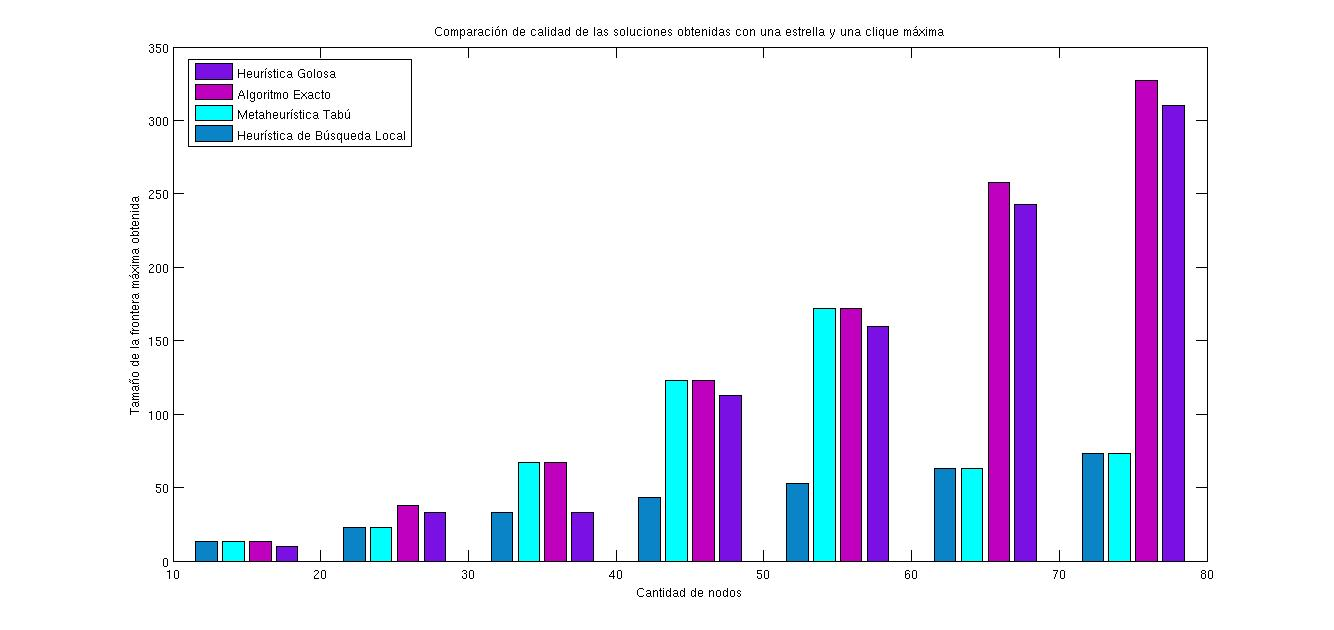
\includegraphics[width=400pt]{../imgs/calidadSolucionesChicas15.jpg}
\caption{Comparación realizada con soluciones chicas con un grafo de tipo Estrella+CMF.}
\end{center}
\end{figure}

En este caso, tenemos una estrella cuyo nodo central no forma parte de la clique de frontera máxima, con lo cual aquellos algoritmos que consideren a los nodos de mayor grado para empezar su ejecución y llegar a un resultado se verán perjudicados por esta familia. Tanto la heurística de búsqueda local como la metaheurística Tabú se ven perjudicadas por la caracterización del grafo, esto se debe a que la heurística parte del nodo de mayor grado y se mueve por una vecindad pequeña y nunca llega a encontrar la CMF que se encuentra a una distancia considerable de la estrella que forma el nodo. En el caso de la metaheurística, lo que sucede es que parte de una solución incial dada por la búsqueda local, con lo cual tiene un punto de partida poco ventajoso que termina provocando que genere un mal resultado. En el caso de la búsqueda golosa, esta se ve beneficiada ya que si bien empieza con el nodo de mayor grado, eventualmente prueba con otros nodos teniendo asá mayor probabilidad de encontrar la clique de frontera máxima. 

 \begin{figure}[H] %[h] Aqui [b] para button [t] para top
\begin{center}
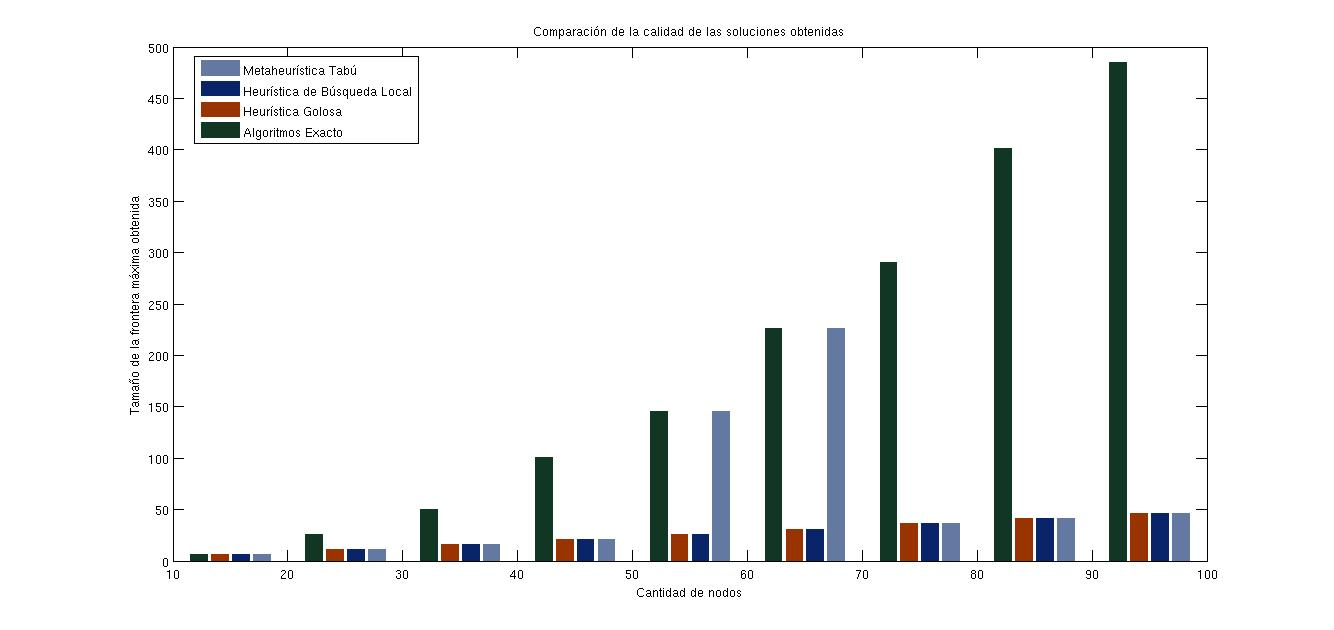
\includegraphics[width=400pt]{../imgs/calidadSolucionesChica14.jpg}
\caption{Comparación realizada con soluciones chicas con un grafo de tipo Estrella+Puente+CMF.}
\end{center}
\end{figure}



En este caso sucede lo mismo que en el anterior, los algoritmos inician en la estrella ya que ésta tiene mayor grado y provoca que nunca se logren mover hasta las soluciones que se encuentran del otro lado del puente que se forma entre la estrella y la estructura que contiene una clique de frontera máxima del otro lado.

 \begin{figure}[H] %[h] Aqui [b] para button [t] para top
\begin{center}
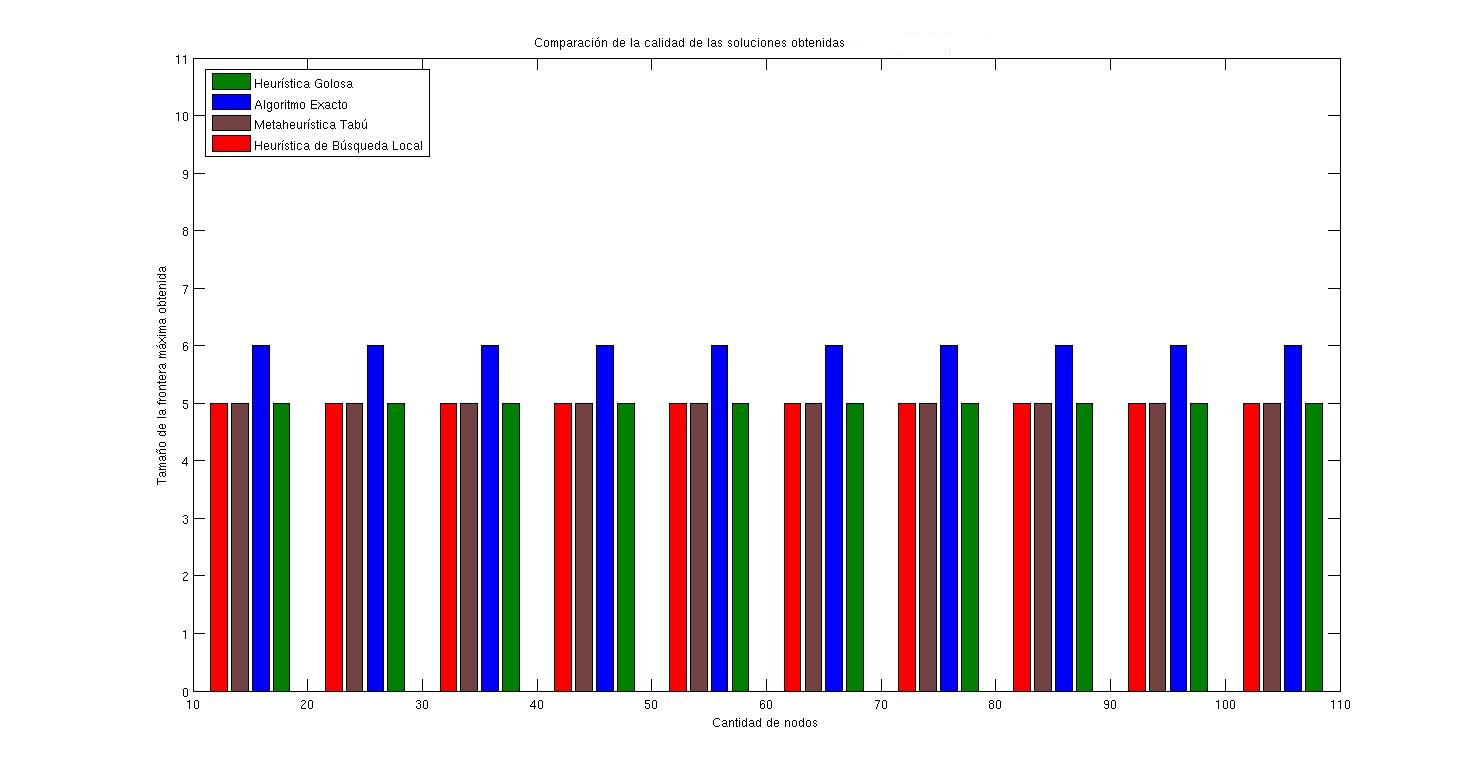
\includegraphics[width=400pt]{../imgs/calidadSolucionesChicas17.jpg}
\caption{Comparación realizada con soluciones chicas con un grafo de tipo Estrella+Puente+Doble Estrella.}
\end{center}
\end{figure}


En este caso, el grafo se caracteriza por contener una estrella que está conectada con dos estrellas. Estas dos estrellas forman una clique de frontera maxima que no contiene al nodo de la primera estrella. Lo que sucede es que la solución de la estrella es parecida a la solucion correcta del problema, pero esta no es la mejor que encuentra el exacto, por eso las heurísticas se quedan con ella mientras que el exacto encuentra la mejor solución entre las estrellas que estan unidas.


 \begin{figure}[H] %[h] Aqui [b] para button [t] para top
\begin{center}
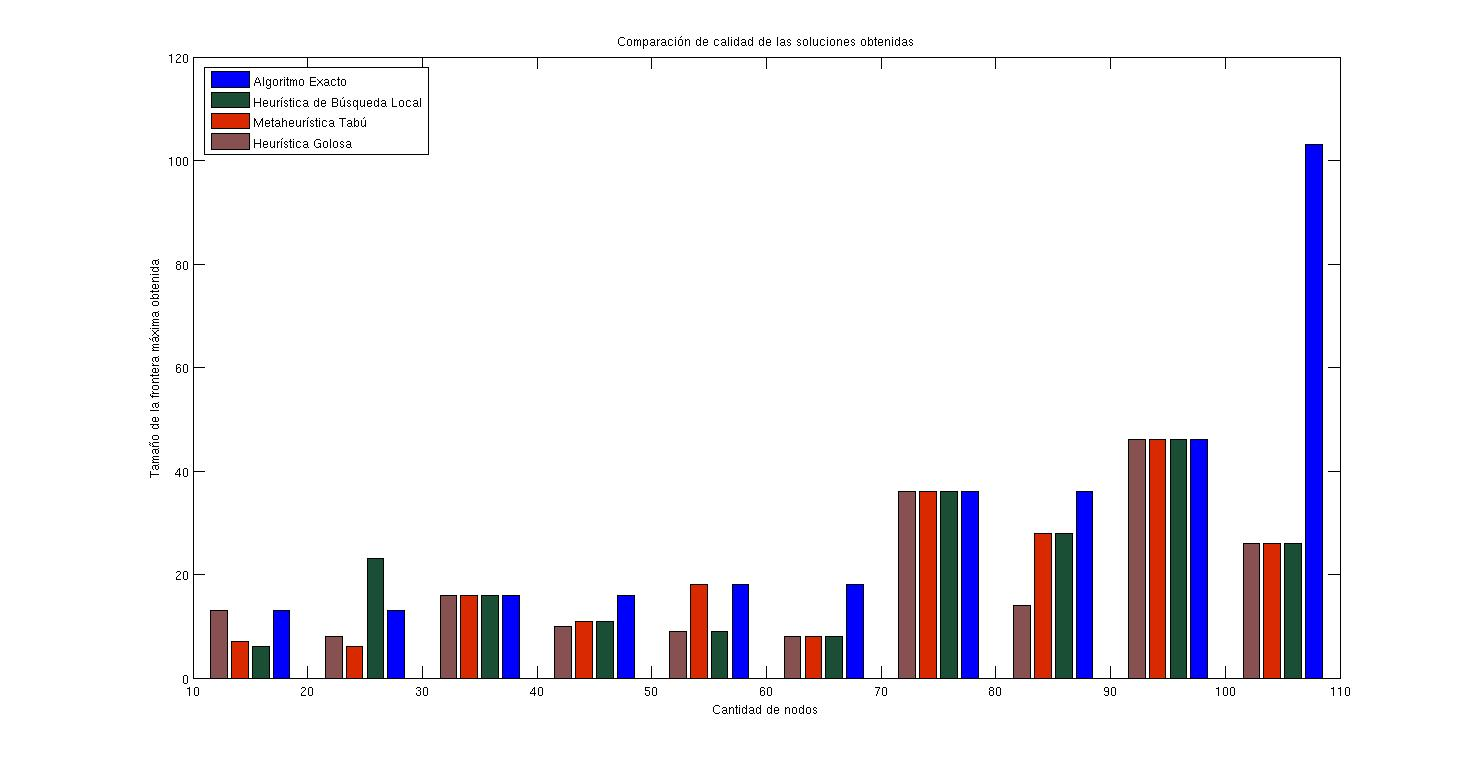
\includegraphics[width=400pt]{../imgs/calidadSolucionesChicas3.jpg}
\caption{Comparación realizada con soluciones chicas con un grafo de tipo Banana Tree.}
\end{center}
\end{figure}

En este caso, tenemos un grafo de tipo banana tree, las heurísticas en la mayoría de los casos obtuvieron soluciones correctas.

 \begin{figure}[H] %[h] Aqui [b] para button [t] para top
\begin{center}
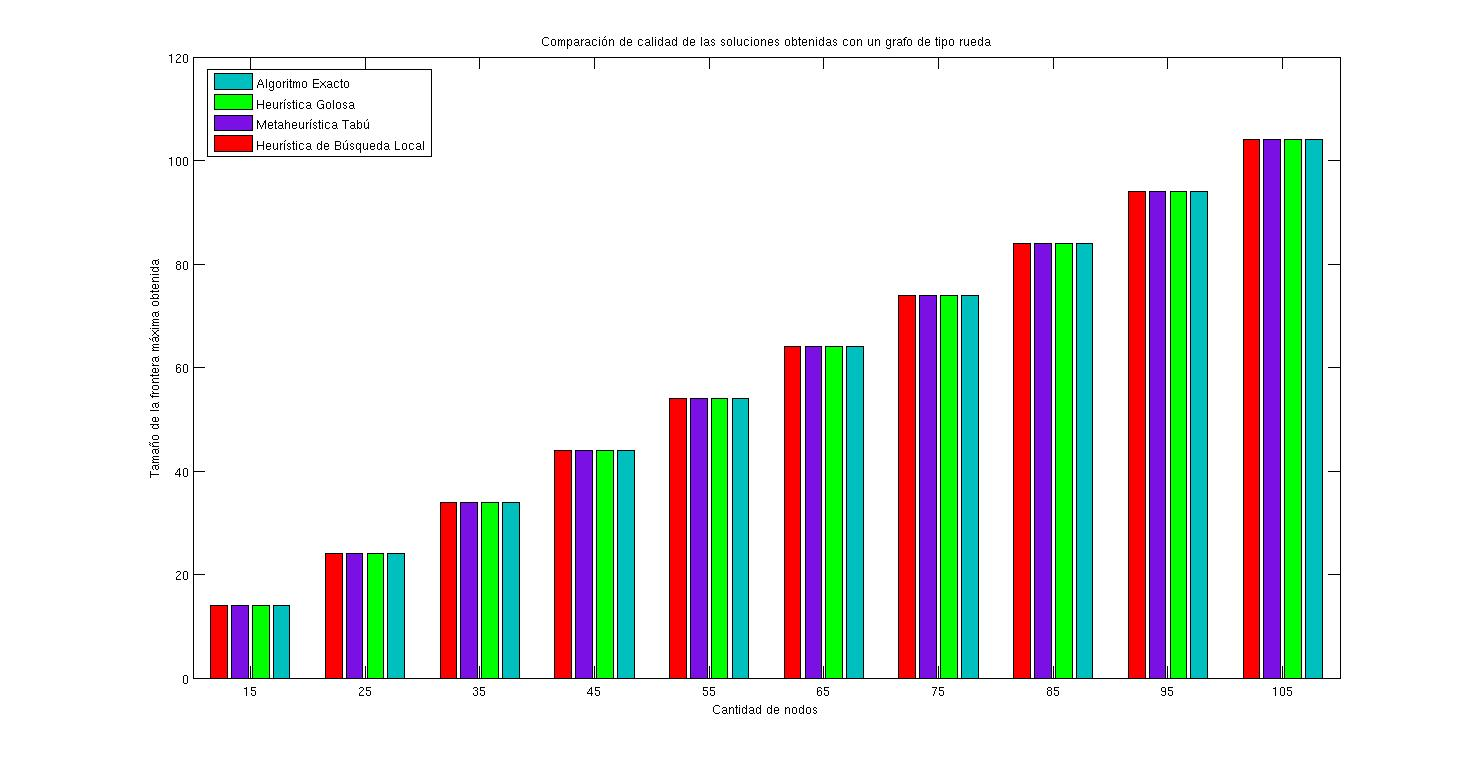
\includegraphics[width=400pt]{../imgs/calidadSolucionesChicas2.jpg}
\caption{Comparación realizada con soluciones chicas con un grafo de tipo rueda.}
\end{center}
\end{figure}

 \begin{figure}[H] %[h] Aqui [b] para button [t] para top
\begin{center}
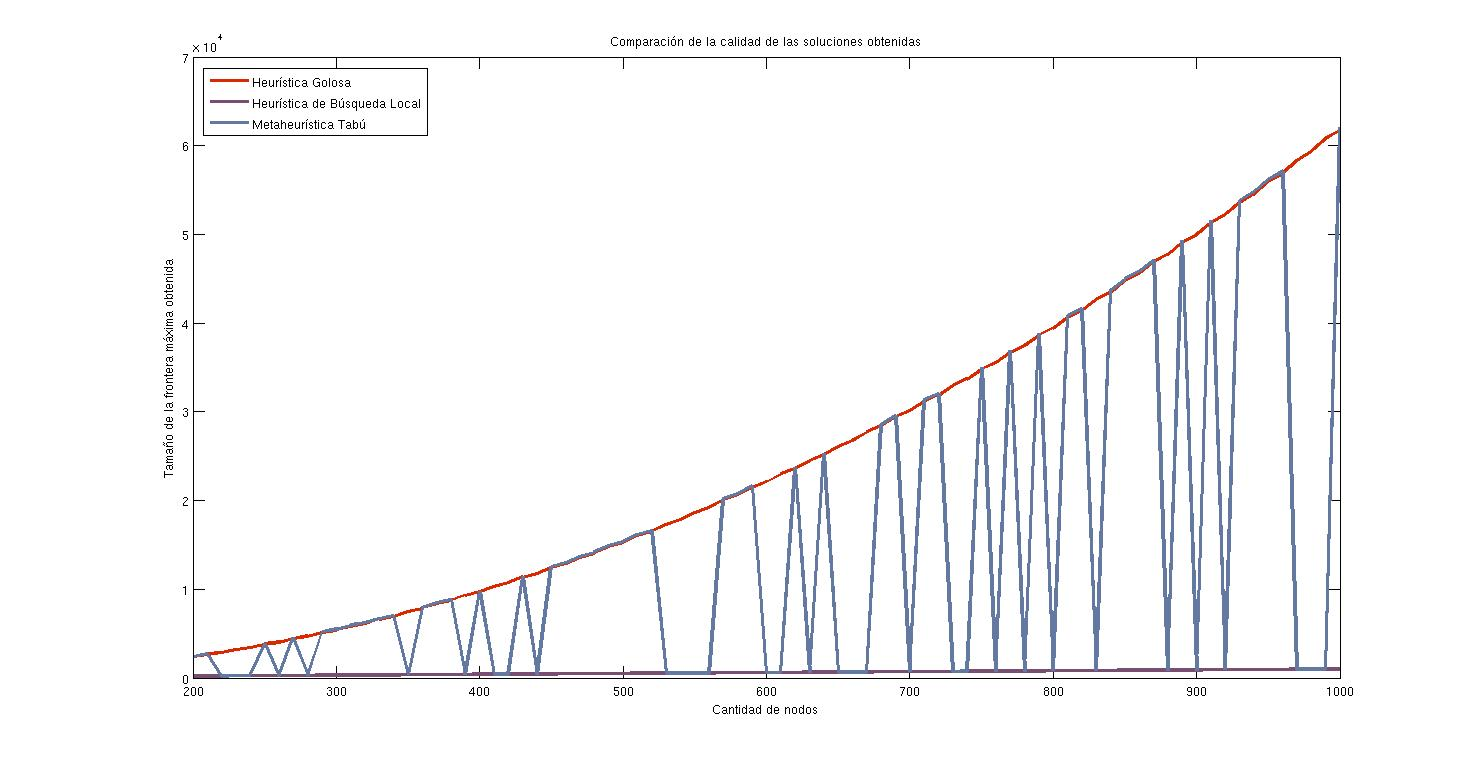
\includegraphics[width=400pt]{../imgs/calidadSolucionesGrandes15.jpg}
\caption{Comparación realizada con soluciones grandes con un grafo de tipo Estrella+CMF.}
\end{center}
\end{figure}

 \begin{figure}[H] %[h] Aqui [b] para button [t] para top
\begin{center}
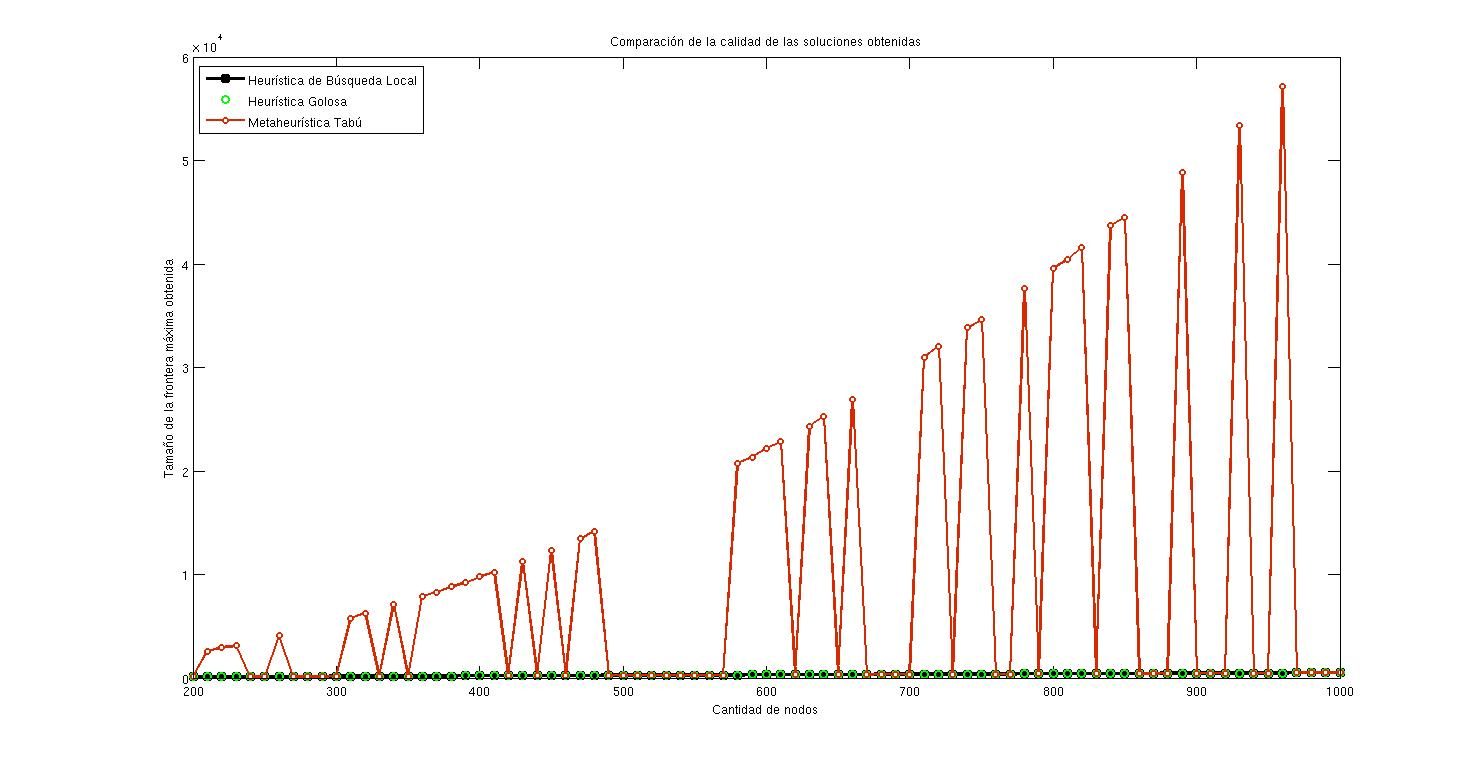
\includegraphics[width=400pt]{../imgs/calidadSolucionesGrandes14.jpg}
\caption{Comparación realizada con soluciones grandes con un grafo de tipo Estrella+Puente+CMF.}
\end{center}
\end{figure}

 \begin{figure}[H] %[h] Aqui [b] para button [t] para top
\begin{center}
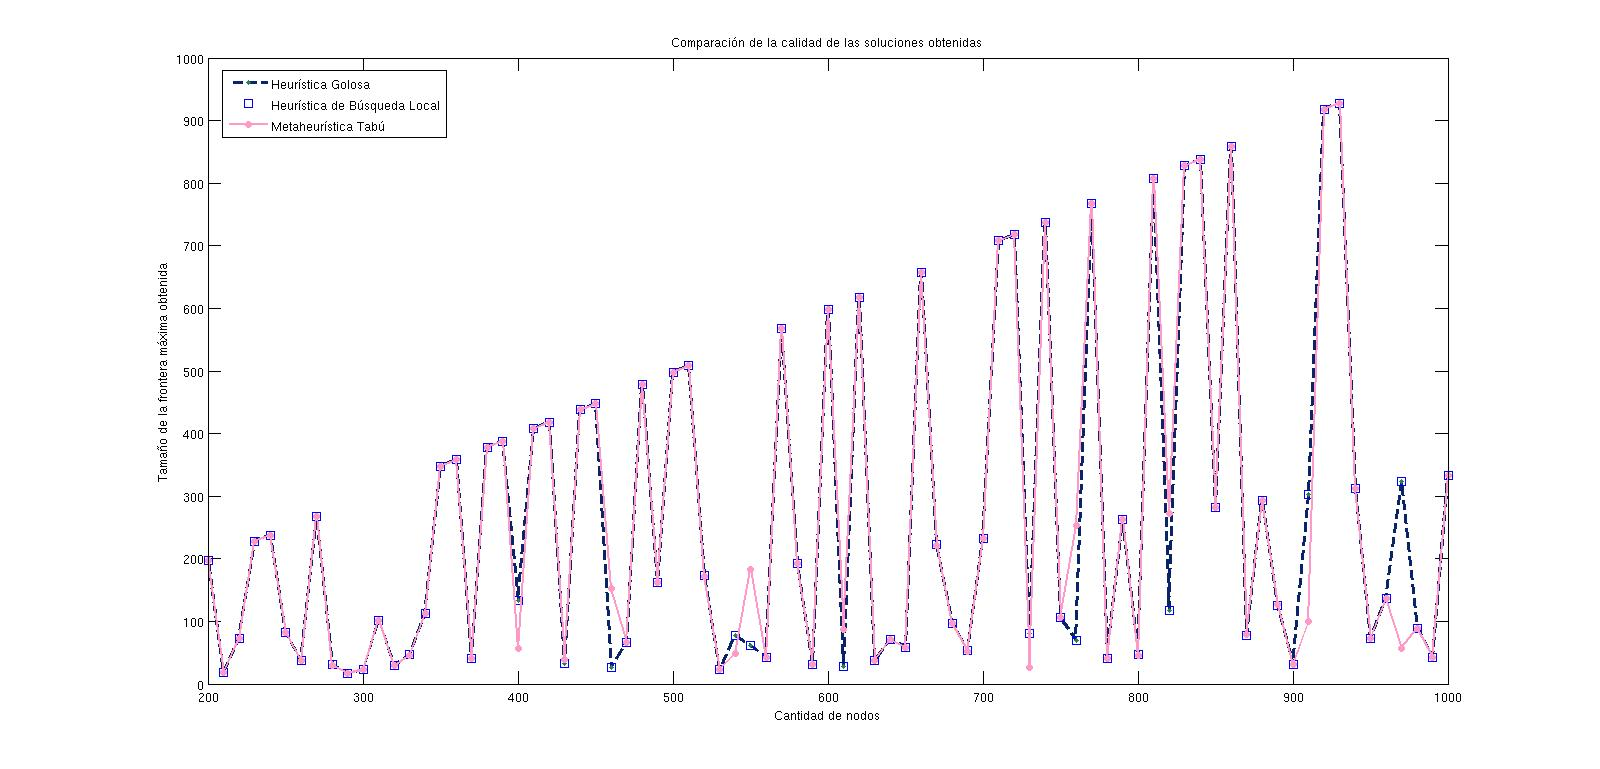
\includegraphics[width=400pt]{../imgs/calidadSolucionesGrandes3.jpg}
\caption{Comparación realizada con soluciones grandes con un grafo de tipo Banana Tree.}
\end{center}
\end{figure}






